\chapter{Keyboard and keys detection design and implementation}
\label{design-and-implementation}

Among the thesis requirements is not only the keys detection to~allow automated typing but also individual keyboard detection so~that a decision if an AIVA unit sees a keyboard screen can be made. For~that reason, a similar approach to~the one described in~the Amazon paper~\cite{amazon-paper} is appropriate. In~this chapter, a three-phase strategy for~automated keyboard typing using current SOTA methods is proposed. Firstly, a keyboard region is detected using the latest YOLO version as~described in~section~\ref{design-keyboard}. Making it a separate subtask, said requirement for~keyboard screen recognition is satisfied. Secondly, keys are detected in~the identified keyboard region which simplifies the recognition in~comparison to~finding the keys in~the whole image. This process presented in sections~\ref{design-keys} and~\ref{design-keys-postprocessing} covers the second and third phases, character detection and post-processing corrections respectively. The whole recognition is reviewed and demonstrated in~the last section~\ref{design-final-detection-process}. Unfortunately, this design cannot be tested against the Amazon's solution as~neither the code nor~the dataset is to~the best of~my knowledge available. This fact makes this work even more contributive, as~no other seems to~currently exist on~the topic.

\section{Keyboard detection}
\label{design-keyboard}
This task can be seen as~a standard object detection with~just a single class to~recognize, a~keyboard. The Amazon researchers used SSD300 neural network with~great results. Since then, a newer, faster and more accurate architecture has been devised which is YOLOv7. While YOLOv7 was briefly introduced in~section~\ref{algorithms-nn-yolo}, as~a selected model architecture, the following section~\ref{design-keyboard-neural-network} describes it in~more depth. Section~\ref{design-keyboard-implementation} demonstrates, how the model was trained and how it can be used.

\subsection{Neural network design for keyboard detection}
\label{design-keyboard-neural-network}
The YOLOv7 paper clearly states that it derives from~the state-of-the-art (SOTA) \hbox{methods} and aims to~improve loss function, label assignment and training~\cite{yolov7}. Hence, the focus is directed on~the incremental changes as~the base architecture of~SOTA YOLO at~the time from~figure~\ref{design-yolo-architecture} is already described in~section~\ref{algorithms-nn-yolo}. YOLOv7 introduces~4~\hbox{major} changes, two architectural (E-ELAN, Model scaling for concatenation-based \hbox{models}) and two trainable bag-of-freebies (Planned re-parameterized convolution, Coarse for~\hbox{auxiliary} and fine for~lead loss).

\begin{figure}[hbt]
    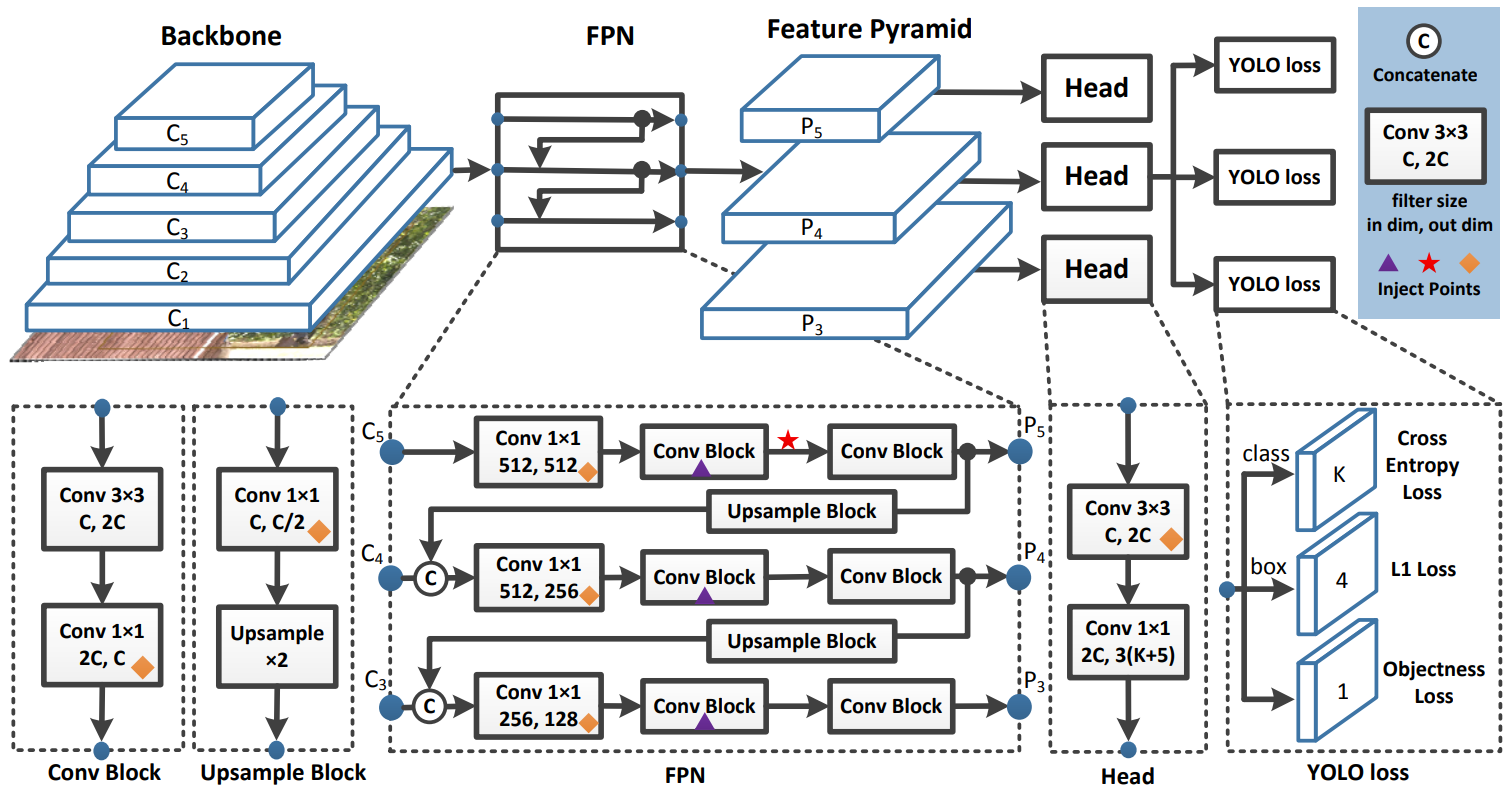
\includegraphics[width=1\textwidth]{img/design/yolov7-architecture.png}
    \caption{General YOLO architecture from~which YOLOv7 derives (taken from~\cite{pp-yolo}).}
    \label{design-yolo-architecture}
\end{figure}

\subsubsection{E-ELAN (Extended efficient layer aggregation network)}
The backbone consists of~E-ELAN computational blocks which depicts figure~\ref{design-yolo-eelan}. These blocks can be stacked and the depth of~the backbone can vary. There were implemented several models (YOLOv7-[X|W6|E6|D6|E6E]) of~different depths which are more accurate but slower respectively~\cite{yolov7}. The blocks are improvements of~ELAN blocks about which not much is known as the paper is not released yet at~the time of~writing of~this thesis. Nevertheless, they are supposed to~help control the longest shortest gradient path to~achieve more effective convergence~\cite{yolov7}. However, they have problems with~scaling and E-ELAN solves it using expand, shuffle and merge feature cardinality~\cite{yolov7}. For~the cardinality expansion, group convolution is used and for~more diverse learning, features of~different groups are shuffled and merged. Thus, more efficient learning is reached while only the inner block architecture is modified and not the outside so the gradient path is unchanged~\cite{yolov7}.

\vspace{-12pt}
\begin{figure}[!hbt]
    \centering
    \subfloat[\centering ELAN]{{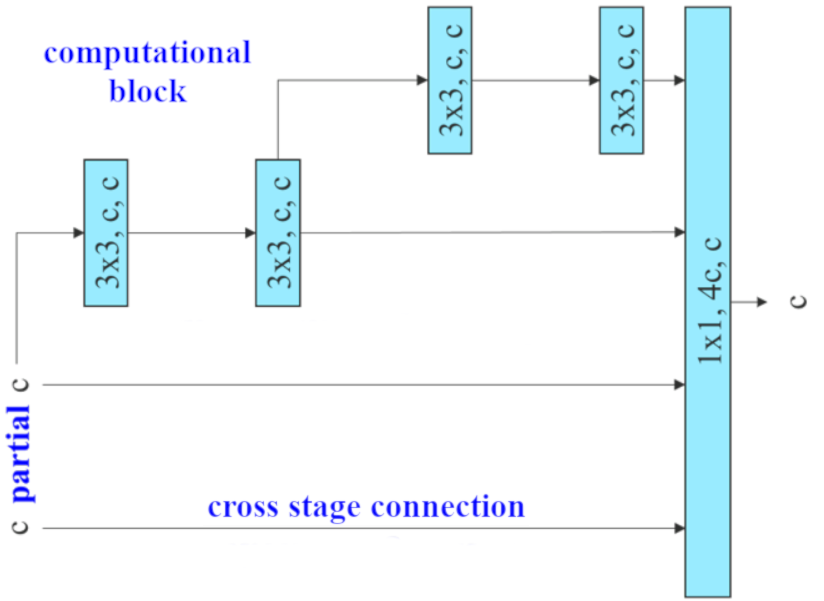
\includegraphics[width=7.45cm]{img/design/yolov7-elan.png} }}
    \subfloat[\centering E-ELAN]{{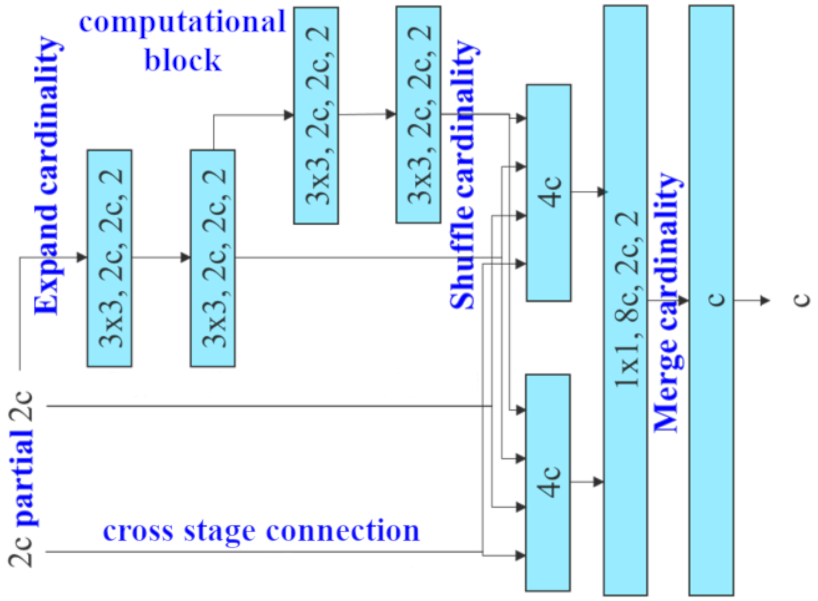
\includegraphics[width=7.45cm]{img/design/yolov7-e-elan.png} }}
    \vspace{-7pt}
    \caption{Difference between the ELAN block upon which YOLOv7 builds and Extended ELAN with~expand, shuffle and merge cardinality blocks (adapted from~\cite{yolov7}).}
    \label{design-yolo-eelan}
\end{figure}

\subsubsection{Model scaling for~concatenation-based models}
When a concatenation-based model is scaled by depth, the output width increases as (a) and (b) in~figure~\ref{design-yolo-scaling} demonstrate. Such changes usually affect the structure of~a model. To~maintain the initial properties of~the original design, a novel scaling method as (c) in figure~\ref{design-yolo-scaling} is~proposed which scales depth and width together~\cite{yolov7}.

\begin{figure}[hbt]
    \centering
    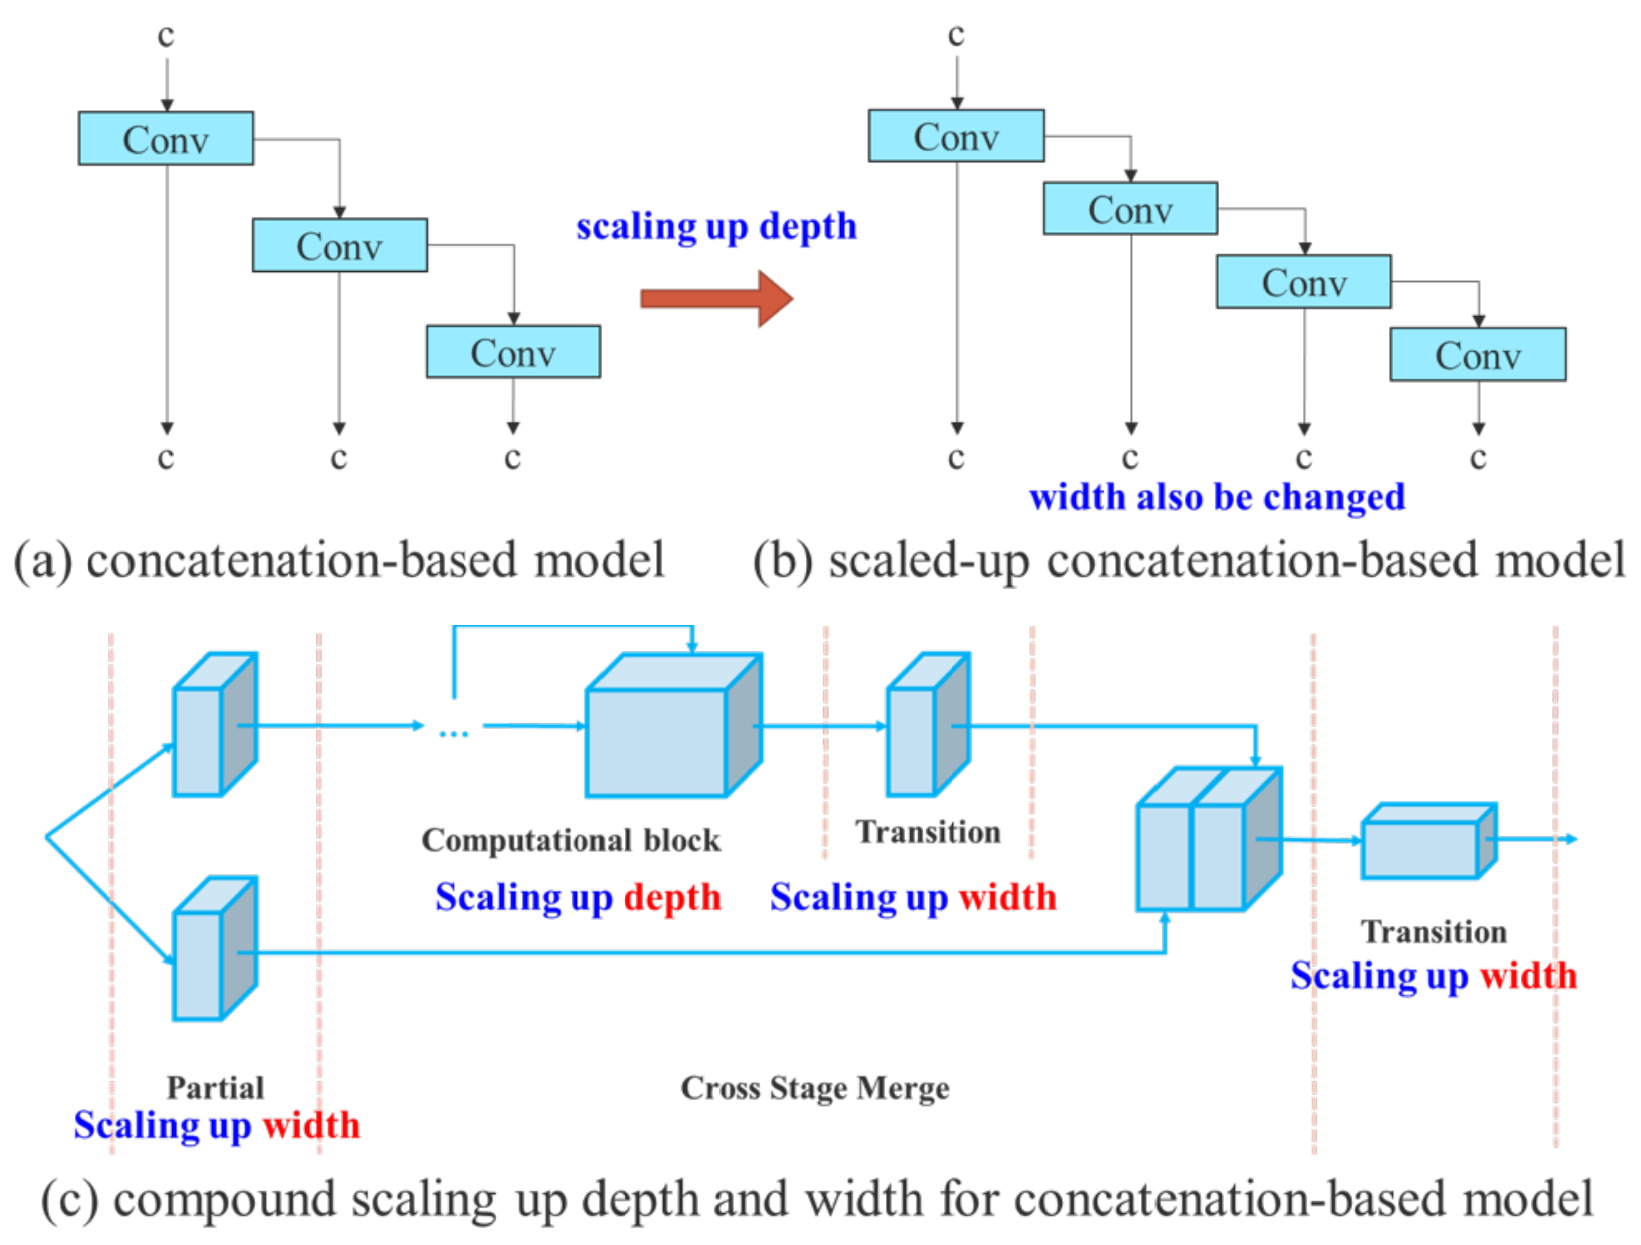
\includegraphics[width=0.9\textwidth]{img/design/yolov7-scaling.png}
    \caption{Depth scaling is required only inside of~a computational block and then the transition layer width is scaled according to~the output channel change~\cite{yolov7} (adapted from~\cite{yolov7}).}
    \label{design-yolo-scaling}
\end{figure}

\subsubsection{Planned re-parameterized convolution}
The purpose of~model re-parameterization is to~merge several computational modules \hbox{during} the inference stage by~averaging weights to~get a more robust module~\cite{yolov7}.
The previous YOLO version used heavily RepConv~\cite{rep-conv} which is a novel highly accurate classification architecture. RepConv combines 3x3 and 1x1 convolutions with~identity connection in~a single convolutional layer~\cite{yolov7}. However, the authors of~YOLOv7 discovered that in~combination with~other architectures such as~ResNet or DenseNet the accuracy is reduced~\cite{yolov7}. They further analyzed re-parameterized convolutions using gradient flow propagation paths in~order to~find out how they should be combined with~different networks. They discovered that RepConv doesn't perform well in~layers with~residual or concatenation connections. Figure~\ref{design-yolo-reparameterization} shows combinations which do or do not work. Hence, they proposed RepConvN (RepConv without the identity) to~be used instead in~such scenarios.

\vspace{-2pt}
\begin{figure}[!hbt]
    \centering
    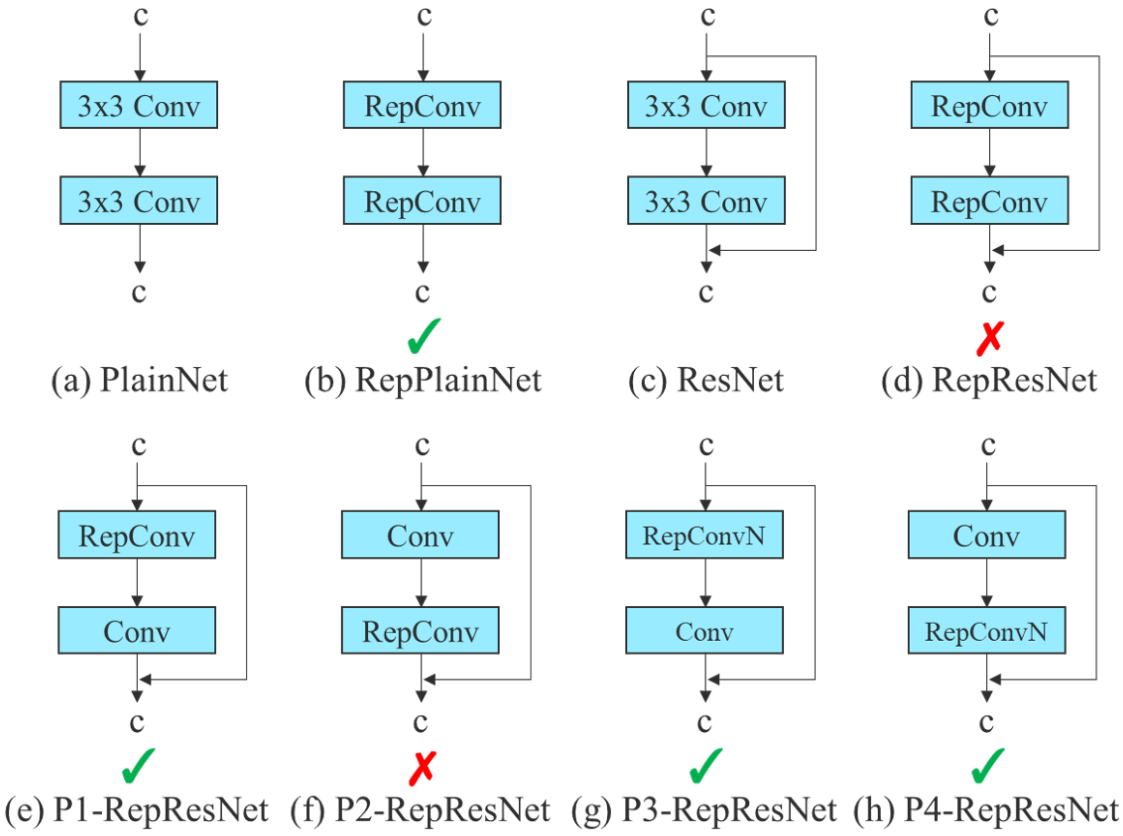
\includegraphics[width=0.7\textwidth]{img/design/yolov7-reparameterization.png}
    \caption{Architectures (not) working with~identity connections (taken from~\cite{yolov7}).}
    \label{design-yolo-reparameterization}
\end{figure}

\subsubsection{Coarse for~auxiliary and fine for~lead loss}
YOLOv7 introduces deep supervision~\cite{deep-supervision} to~the YOLO architecture. Figure~\ref{design-yolo-heads}~(a) depicts how auxiliary heads are added to~the model. In~general, the lead heads
are still responsible for~the final prediction, the auxiliary heads just help with~the training. While figure~\ref{design-yolo-heads}~(b) shows the popular approach at~the time that both heads make their own prediction, the proposed method in~YOLOv7 is to~guide both heads by~lead head prediction using (c) and (d) assigners~\cite{yolov7}. The paper describes them followingly. Lead guided assigner takes ground truth and lead head predictions and generates soft labels which are used as~targets for~both lead and auxiliary heads during the training. This way, the shallower auxiliary head can learn the predictions from~a more accurate lead head and the lead head can in~turn focus on~not yet learnt information. Coarse-to-fine lead head guided assigner also uses lead head predictions but creates~2~sets of~labels. Fine labels are the same as~soft labels in~the previous assigner. Coarse labels are generated with~lesser constraints for~positive sample assignment as~auxiliary heads have weaker learning capabilities and this can help to~avoid information loss.

\begin{figure}[hbt]
    \centering
    \subfloat[\centering Model with auxiliary heads]{{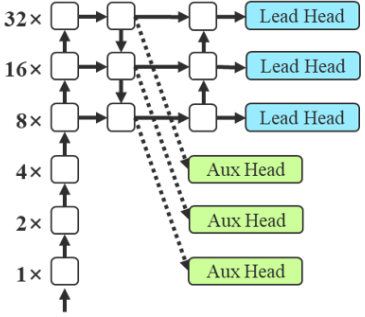
\includegraphics[width=6cm]{img/design/yolov7-heads-auxiliary-heads.png} }}
    \subfloat[\centering Independent assigner]{{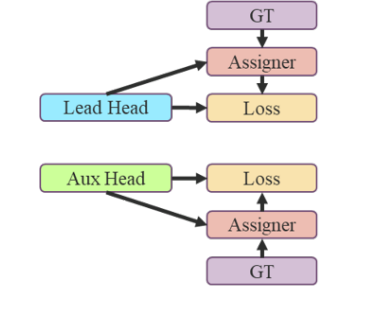
\includegraphics[width=6cm]{img/design/yolov7-heads-indipendent-assigner.png} }}
    \\
    \subfloat[\centering Lead guided assigner]{{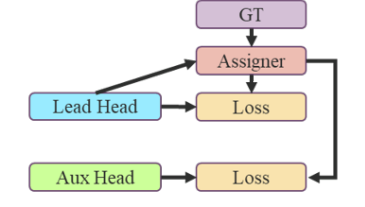
\includegraphics[width=6cm]{img/design/yolov7-heads-guided-assigner.png} }}
    \subfloat[\centering Coarse-to-fine lead guided assigner]{{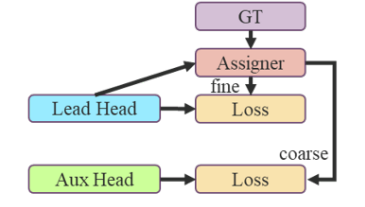
\includegraphics[width=6cm]{img/design/yolov7-heads-coarse-to-fine.png} }}
    
    \caption{Deep supervision adds auxiliary heads to~the middle of~a model (a). Label assigners are usually independent for~both lead and auxiliary heads (b), but YOLOv7 introduces assigners for~both heads (c, d)~\cite{yolov7} (adapted from~\cite{yolov7}).}
    \label{design-yolo-heads}
\end{figure}

\subsection{Training and usage of the detector}
\label{design-keyboard-implementation}
The YOLOv7 paper implementation is available on~GitHub\footnote[1]{\url{https://github.com/WongKinYiu/yolov7}} and is written using \hbox{PyTorch}. Hence the implementation of~the whole thesis is in~Python as well. The usage of~YOLOv7 is very straightforward and is shown by~algorithm~\ref{yolov7-code}. Firstly, one must install Python requirements (dependent libraries) either globally or in~a virtual environment, which is recommended. Secondly, a training run can optionally be initialized in the Weights \& Biases platform which the YOLOv7 project uses for logging and metrics collection. In~the code~\ref{yolov7-code}, this is done from Python while the other commands are for the command line, which is legit if using a Jupyter notebook for instance. Lastly, training itself can start.

\begin{algorithm}[!hbt]
    \begin{lstlisting}[language=bash, keywords={python3, pip3, source}]
# set virtual environment not to install dependencies globally
python3 -m venv yolov7-env
source yolov7-env/bin/activate
# install requirements
pip3 install -qr requirements.txt
# Weights & Biases connection - optional and in Python code
wandb.login(key="API KEY OF YOUR ACCOUNT")
wandb.init(project="yolov7", name="yolov7-keyboards")
# train
python3 train.py --img-size 640 640 --cfg cfg/training/yolov7.yaml
--hyp data/hyp.scratch.custom.yaml --data data/keyboards-local.yaml
--name yolov7-keyboards --weights '' --batch-size 16 --epochs 30
    \end{lstlisting}
    \caption{Bash and Python code for running YOLOv7 training}
    \label{yolov7-code}
\end{algorithm}

\begin{description}[topsep=0pt,itemsep=-1.5pt,partopsep=6pt]
  \item[-{}-img-size] This parameter means that both training and testing images have input size of~640x640 pixels. The actual images can have any size, but they will be scaled or padded to~this size as the model works with 640x640~images. There are network configurations even for 1280x1280 input images, which are more accurate, but also bigger, slower and unnecessary for this task. The base~640x640~is more than twice the resolution of~the SSD300 which is proven to work well.
  \item[-{}-cfg] The authors prepared several network configurations. The \emph{yolov7.yaml} file describes the paper architecture. Then another significantly smaller and faster variant, designed for microcontrollers and such, is called yolov7-tiny. The last one still for~640x640~input images is called yolov7-x, which is like the~1280x1280~models more accurate at~the cost of~size, speed and computation resources. These~3~were trained, tested and the most appropriate was selected. There are another 4 variants (W6, E6, D6, E6E) for~1280x1280~input images which were not considered for~this task.
  \item[-{}-hyp] This parameter describes training hyperparameters such as~learning rate, weight decay, momentum etc. These were not changed for~the training.
  \item[-{}-data] This one specifies the training and testing data along with the number of~classes and class names. The model is trained on the dataset described in~chapter~\ref{dataset-keyboards}.
  \item[-{}-name] A name under which the training results are saved.
  \item[-{}-weights] Specification of pre-trained weights which can be used for~finetuning or resuming a halted training.
  \item[-{}-batch-size] Size of the mini-batch that should be used during the training.
  \item[-{}-epochs] Number of epochs the training should run for.
\end{description}

To~achieve optimal training results, several argument settings were examined. One was whether to use a pre-trained model on~the COCO17 dataset, which includes keyboards in~a scene. For~a demonstration of~the difference between finetuned and not finetuned training, chart~\ref{nn-finetuned-vs-notfinetuned} shows the comparison of~the development of~mAP@.95 metric during~30~epochs using batch size~32. After the first epoch, it is clear that the pre-trained model knows something already. However, the drop after the second epoch suggests that it forgot \hbox{everything} and started training anew. The beginning of~the finetuning is quite volatile and after stabilization, it goes hand in hand with normal training. During the not finetuned training, on~the contrary, the improvements are steady. A~conclusion can be drawn, that the finetuning does not add any value to~the training results, and hence can be omitted.

\vspace{-9pt}
\begin{figure}[hbt]
    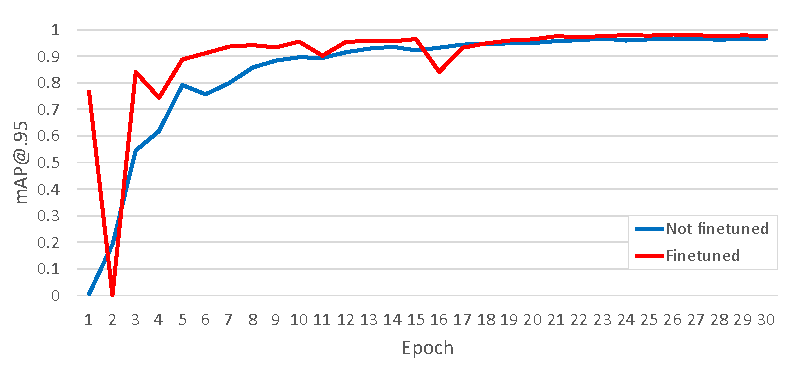
\includegraphics[width=1\textwidth]{img/design/nn-finetuned-vs-notfinetuned.pdf}
    \vspace{-20pt}
    \caption{A~comparison of~mAP@.95 development on~validation data during training a new model and finetuning an existing one proves that finetuning does not bring any benefit.}
    \label{nn-finetuned-vs-notfinetuned}
\end{figure}

Another argument selection concerns the batch size. Usually, a power of~2~is selected, namely one of~32~or~64. The YOLOv7 default is set to~16, so it was compared to~32~if it brings any improvements. Chart~\ref{nn-batch-16-vs-32} displays the difference. Lower batch sizes generally slow down the training as the weights are updated more often and the vectorization potential is reduced. Conversely, the more frequent weight updates might (not a rule) improve accuracy.

\vspace{-9pt}
\begin{figure}[!hbt]
    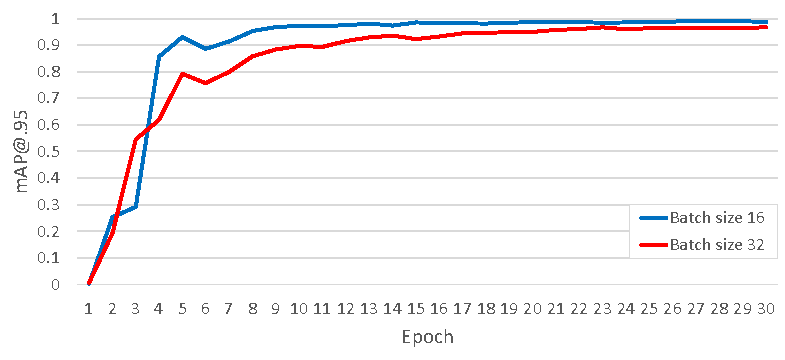
\includegraphics[width=1\textwidth]{img/design/nn-batch-16-vs-32.pdf}
    \vspace{-20pt}
    \caption{A~comparison of~mAP@.95 development on~validation data during trainings with batch sizes~16~and~32~clearly shows that batch size~16~achieves better results.}
    \label{nn-batch-16-vs-32}
\end{figure}

The remaining parameter, the number of epochs, was set to~30~for~visible reason in~both charts~\ref{nn-finetuned-vs-notfinetuned} and~\ref{nn-batch-16-vs-32}. Most of~the learning occurred in~the first~10~epochs, in~the next~10 there were significantly smaller improvements and in the last~10 it stabilized completely. In~this manner were trained all~3~640x640~models (yolov7-tiny, yolov7, yolov7-x) and the results are further discussed in~chapter~\ref{evaluation}. Full training results are available on~the attached medium~\ref{Appendix-A}.

Once the model is trained, the YOLOv7 project provides \emph{detect.py} script for the \hbox{actual} detection. However, this is not usable in~a custom solution. Therefore, Python pseudocode~\ref{yolov7-detect} demonstrates the model usage. Firstly, PyTorch loads the model and sets it from training to~evaluation mode. Secondly, the given image is transformed into~the detector's format, which means scaling and adding padding to~640x640 size and normalizing color values from~0-255~to~\hbox{0-1}. Then the model makes its predictions on which the non-maximum suppression method is applied. By~default, only the detections with a higher confidence score than~0.5~and only the best from the overlapping ones (iou = intersection over union threshold) are selected. Lastly, the detected bounding boxes are scaled back to the original image size.

\begin{algorithm}[!hbt]
    \begin{lstlisting}[keywords={def, return}, xleftmargin=20pt, numbers=left]
def detect(model_path, img, confidence=0.5, iou=0):
    model = torch.load(model_path)
    model.eval()
    input_img = prepare_img(img)
    predictions = model(input_img)
    predictions = non_maximum_suppresion(predictions, confidence, iou)
    predictions = scale_to_original(predictions, img)
        
    return predictions
    \end{lstlisting}
    \caption{Python pseudocode for a detection function using YOLOv7 model}
    \label{yolov7-detect}
\end{algorithm}

\section{Keys detection}
\label{design-keys}
Recognition of~keys on~a keyboard is the most challenging part of~this work. The Amazon research team used modified SSTD (Single Shot Text Detector)~\cite{sstd} architecture. SSTD serves for~text detection in~a scene image. However, it only finds text regions and does not recognize the text meaning~\cite{sstd}. The main modifications made were output change to~support multiple character classes and addition of~a non-maximum suppression layer so that it does not try to~join characters into~words~\cite{amazon-paper}. Nonetheless, I found~2~issues with~this approach. One of~them is that I do not see the point in~using a scene text detector and reducing its capabilities. Firstly, there is no real-world scene as~keyboards are basically just characters on~a background with some UI design. Secondly, the attention module for~text prediction in~SSTD misses the mark once the task is reduced to~single-character detection. The other problem is for~example the space key. In~many cases, the key is empty without any icon or \say{space} word. This leads~to a realization that just character recognition is not sufficient and a method for~the actual key (not its text) detection must be included. The proposed solution is to~use the current SOTA YOLOv7 for~the character recognition according to section~\ref{design-nn-chars} and Canny edge detector described by~section~\ref{design-classical-algorithms} for~checking the positions of those keys that have predefined locations such as~some special keys. This way there can be predicted potentially missing or incorrectly detected keys.

\subsection{Neural network design for character detection}
\label{design-nn-chars}
As~mentioned in~sections~\ref{algorithms-nn-yolo} and~\ref{design-keyboard}, YOLOv7 is the current SOTA in~object detection so it was selected for~this task as~well. Text detectors like SSTD or other OCRs usually aim at~detecting words or even sentences in~a scene. In~order to~achieve this, attention mechanism and other text-specialised methods are used~\cite{sstd}. This would make them more suitable models if text detection was the objective. Nevertheless, single-character detection is meant to~be solved. Consequently, the contextless feature of YOLOv7 is beneficial as it does not try to~merge the characters into~words.

The model was trained on~640x640 images from the generated dataset described in~section~\ref{dataset-characters}. To~fully disclose, there was no illusion of counting on great accuracy results, especially for~special characters such as dots, commas, semicolons etc. as~for~instance a semicolon can be recognized as~independent dot and comma. Many other examples like this one can be thought~of. A~lot of~such detection inaccuracies are solved by~the detection correction post-processing mechanism~\ref{design-keys-postprocessing}. Moreover, to~remind the task specification from section~\ref{introduction-expectation}, the main focus is on~alphanumeric characters. The endeavor to~recognize special characters as~well was made but as a secondary objective with a separate evaluation.

Concerning the actual training of~the model, it is the same as for~the keyboards described in~section~\ref{design-keyboard-implementation} with just~2~subtle differences. The first one is an increased number of~epochs to~50~as there are~99~classes and it takes longer to~train. The second one is a modification of~the original hyperparameters configuration file. Flipping of~objects during training was turned off because for example flipping the~left parenthesis results in~the right one which is a different class. Moreover, changes in~color, saturation and scale were reduced as it was already the subject of~dataset generation. The detector is further evaluated in~chapter~\ref{evaluation}.

When it comes to the usage of~the model to detect characters on~actual keyboards, an inconvenience comes up. Keyboards are usually very wide which is adversarial to the scaling. Let's assume a common scenario with a digital display where the keyboard covers about half of~the screen. On~the target full-HD image it would mean 1920x540 keyboard resolution which would scale down to 640x180. This results in~significant information loss and~2/3~of~the image under detection being padding. Instead of~simply scaling the image down, it is split and several detections are run. Full-HD width 1920px is convenient as it is exactly~3~times the width of~the detector's input. However, a certain overlap is necessary to avoid cutting a character in~half during the split. The overlap used is 64px which is the biggest font size on~which the model was trained. Consequently, the input image is split into several images which fit the 640x640 block. In~the case of the full-HD image with the overlap included, it is~4~images, but the algorithm is flexible so it is always split into the right number and no information is lost. The splitting is done only on the \emph{x}-axis, because 640px height is not expected to be exceeded or just slightly. Should it be significantly larger, the information loss during the scale-down is completely acceptable. Of~course, multiple detections influence negatively the performance. Nevertheless, the images can be batched and run in~a single computation just as another dimension of~the matrix. Furthermore, as YOLOv7 is a real-time detector with detection time in~milliseconds depending on~the machine, the slow-down is tolerable for~the use case.

\subsection{Key regions proposal using classical computer vision techniques}
\label{design-classical-algorithms}
The examples provided in~section~\ref{algorithms-classical} show that both edge detection and thresholding can produce satisfying results. Due to their similar results and no obvious reason why one should be better than the other, the Canny edge detection technique was chosen as the classical algorithm candidate because it is a bit simpler to use. The thresholding requires slightly more operations. Owing to~the simplicity and speed of this method, the initial idea was to use it as~a region proposer and then a classifier could be used to~recognize the characters. This strategy seemed to~solve it all. It could handle empty keys like space and achieve outstanding accuracy as~there already exist many character classifiers and datasets such as~MNIST. Despite~of~initial successes, though, two major issues concerning both edge detection and thresholding arose. The first one is contour computation depicted by~figure~\ref{canny-countour-problem}. As~there can be seen, many smaller regions were often detected instead of a full key. This might happen when an edge is not complete and has spaces in it which compromise the contour. Another complication is the detection of~both a key and a character. Which one to~use? The inner box (character) would be more suited for~the subsequent classification but then which to~choose e.g. between \emph{t} and~\emph{5}? It could be decided based on~the size but what if for~instance \emph{j} has its dot isolated or another contour error occurs? Too many inconvenient scenarios emerge which does not play well for~this strategy.

\begin{figure}[hbt]
    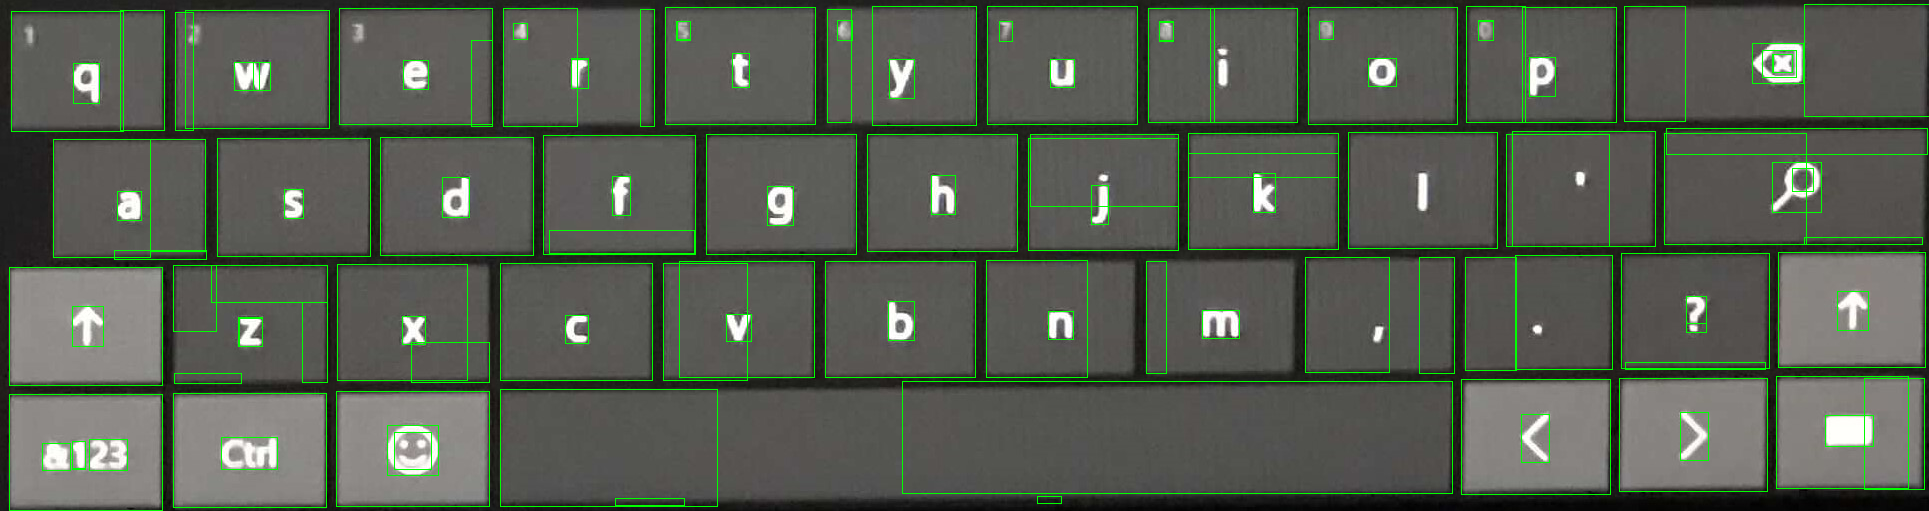
\includegraphics[width=1\textwidth]{img/design/canny-contour-problem.png}
    \caption{Contour computation problem in~edge detection region proposal}
    \label{canny-countour-problem}
\end{figure}

The second issue is the variety of UI designs that can create a huge amount of false positives. Something similar might happen with a background in a transparent keyboard. An example of such UI design is shown in~figure~\ref{canny-ui-problem}. Image (a) shows a car infotainment keyboard with vertical lines going to the background at~the bottom of the keyboard. This, however, renders the contour computation completely useless as~image (b) demonstrates. There would be a huge amount of~bounding boxes produced not only for the bottom vertical lines but also for the horizontal lines under the characters symbolizing the keys.

\begin{figure}[!tbh]
    \centering
    \subfloat[\centering Original image]{{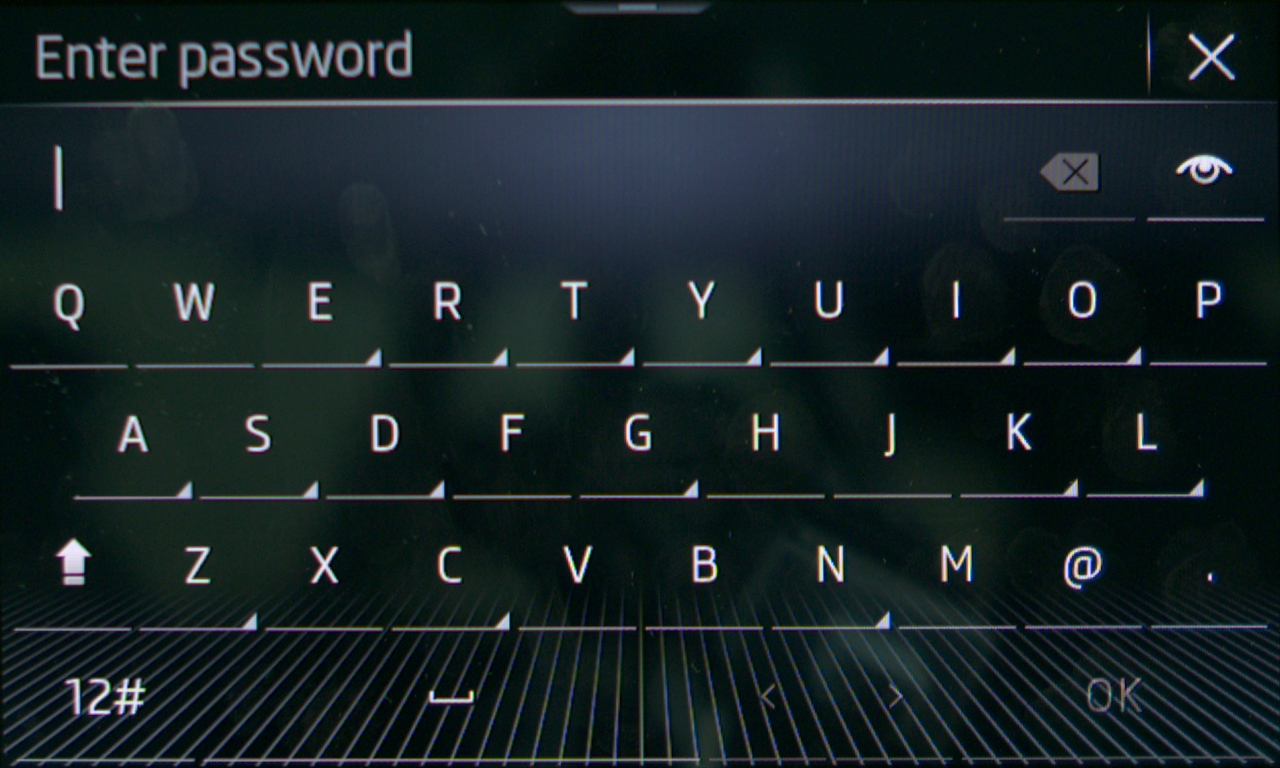
\includegraphics[width=7.45cm]{img/design/canny-ui-skoda-orig.jpg} }}
    \subfloat[\centering Binary image after Canny edge detection]{{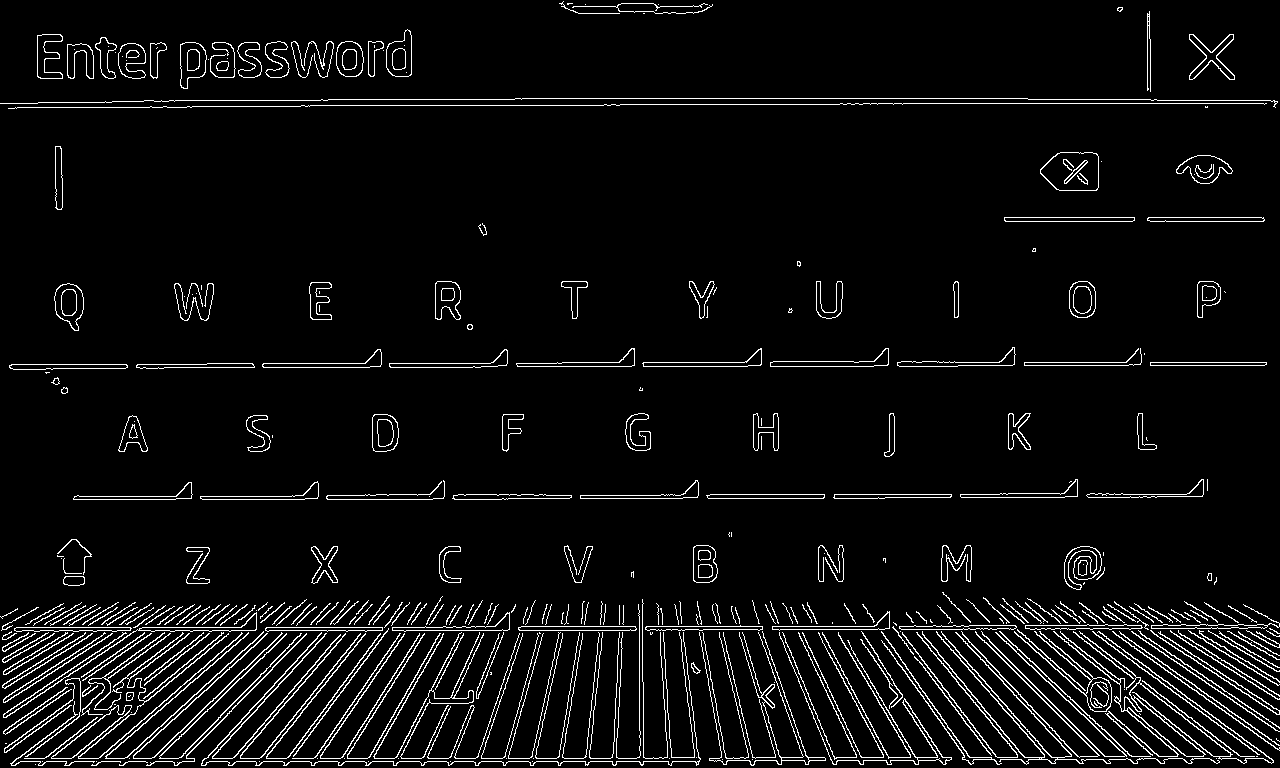
\includegraphics[width=7.45cm]{img/design/canny-ui-skoda-binary.png} }}
    %\vspace{-6pt}
    \caption{UI keyboard designs can generate too many edges.}
    \label{canny-ui-problem}
\end{figure}

 What is more, it would be throwing out~the progress in~the object detection field and returning to~two-stage detectors. For these reasons, a detection neural network approach was opted for in~the end. Nevertheless, Canny edge detection is still run in~parallel as a supplementary bounding box provider of potential keys for the post-processing phase. Firstly, it costs almost nothing as it is computed parallelly. Secondly, the neural network does not solve the empty space key problem. If there is no icon or word on~the space key or it is not detected, the Canny edge detector might detect the key's rectangle. The same goes for other special keys such as shift if the icon or word is not detected. Which special keys are double-checked and how is the subject of section~\ref{postprocessing-canny}, the current section concentrates on~how the bounding boxes of~candidate key regions are obtained. The Python pseudocode~\ref{canny-pseudocode} describes the process.

\begin{algorithm}[!hbt]
    \begin{lstlisting}[keywords={def, return}, xleftmargin=20pt, numbers=left]
def run_canny_detection(img):
    img = clahe(img)
    img = cv2.cvtColor(img, cv2.COLOR_BGR2GRAY)
    img = cv2.bilateralFilter(img, 8, 30, 70)
    img = cv2.Canny(img, 25, 50)
    contours, _ = cv2.findContours(img)
    bboxes = convert_contours_to_bboxes(contours)

    return bboxes
    \end{lstlisting}
    \caption{Python pseudocode for Canny edge detection using OpenCV}
    \label{canny-pseudocode}
\end{algorithm}

Before the actual edge detection is performed, several image modifications to improve the detection results are done. To~highlight the edges a bit more, the clahe~\cite{clahe} contrast enhancing method is used. Then the image is transformed into a grayscale representation. Finally, bilateral filtering~\cite{opencv-library} is used to reduce noise while keeping edges. The second parameter~8~specifies the pixel neighborhood distance which influences the other parameters. The third one~30~is a relative measure of how much are the colors mixed together. The last parameter~70~is a relative measure of~how much the pixels influence each other taking the color into account as well. The subsequent Canny method accepts the lower and higher thresholds described in section~\ref{algorithms-classical-canny} and outputs a binary image with edges. Contours are computed for the edges and converted to~[x1, y1, x2, y2] bounding boxes.

\section{Post-processing of keys detection results}
\label{design-keys-postprocessing}
This is the third and final stage to~the whole process and it has several subtasks. In~general, it tries to validate the detected keys, correct any inaccuracies and fill in the undetected keys. For this purpose, supported layouts, keywords and other patterns are predefined as~rules and the detected characters are checked against these rules. To~make an example, let's assume we have a detected~\say{r} character and we want to check if it is the~\say{r} in~a qwerty row. The rule for this scenario says there should be \say{qwe} left of~the character and \say{tyuiop} right of~it. If there is a sufficient number of~matching characters in~the correct order, the check passes. Then the distances between characters are obtained and missing undetected characters can be computed or inaccurate bounding boxes corrected. Any sequence can be checked in~such a manner and the following sections describe each part in~more detail. The rule checking is the same, though. Before diving into the specifics, algorithm~\ref{postprocessing-algorithm} demonstrates the whole process.

\begin{algorithm}
    \hspace*{\algorithmicindent} \textbf{Input} Recognized characters \emph{chars} and Canny edge detection results \emph{canny\_bboxes} \\
    \hspace*{\algorithmicindent} \textbf{Output} Processed and accepted keys
    \begin{algorithmic}[1]
    \STATE $processed\gets \{\}$
    \STATE $rows\gets find\_rows(chars)$
    \STATE $check\_pinpad(rows, processed)$
    \STATE $check\_keywords(rows, processed)$
    \STATE $layout\gets check\_layout(rows, processed)$
    \STATE $check\_number\_line(rows, processed, layout)$
    \STATE $check\_icons(rows, processed, layout)$
    \STATE $check\_special\_characters(rows, processed, layout)$
    \STATE $guess\_special\_keys\_from\_canny(processed, canny\_bboxes, layout)$
    \STATE $correct\_capitalization(processed)$
    \end{algorithmic}
    \caption{High-level key detection post-processing process}
    \label{postprocessing-algorithm}
\end{algorithm}

In~the beginning, none of~the detected characters is accepted yet. Every detection is added to~the result only if it matches a rule. To have an idea about the detection placements and their relationships, they have to be organized into a structure. Simple rows were selected. For two bounding boxes to be in~the same row, they must overlap on~the \emph{y}-axis for at~least~50~\%. The rows are ordered bottom up and characters in~a row are ordered left to right by~the \emph{x}-axis. This is sufficient because keyboards are basically grids and it is easy to check a character's row for a sequence rule. Next, a pin-pad layout existence is checked. This is necessary to do before a layout recognition because otherwise the common alphabetical characters below or next to the pin-pad numbers could be incorrectly viewed as an alphabetical layout. Once it is clear whether a pin-pad keyboard is being processed or not, qwerty vs. alphabetical layout recognition can begin. Nevertheless, to reduce the number of~characters in~the layout recognition, keyword detection precedes it. Following is a 1-9 number line check, which is a very common sequence on~keyboards. Notice that zero is omitted as it can be either at~the start or end (more usual) of~the sequence. Then, special key icons and special characters are processed. These are basically the remaining detection results and with them ends any positional or correctional processing of~the character recognition. Thereafter, the Canny edge detection results are used to guess undetected special keys based on~the already detected ones. Finally, correction of~lower vs. upper case is performed. A~lot of characters such as x vs. X or s vs. S etc. are hardly distinguishable from each other and the character detector can easily make a mistake. For that reason, discrimi\-native characters \say{abdehmnqrty} whose lower and upper variants differ based on~intuition and character detector results are selected. All characters are set to the prevailing case among the discriminative characters. It is worth mentioning that at~the very beginning of~the post-processing, all characters are transformed to lowercase for easier manipulation and the information about their original case is saved for this part.

\subsection{Numbers processing}
\label{postprocessing-numbers}
There are~2~numbers-processing tasks performed. At~the very beginning of~the post-processing, a search for~a pin-pad layout is run. The \emph{x}~coordinates of~all numbers are checked against each other if they overlap to~find potential columns. The column patterns are 147, 258, and 369 so if for instance 4 overlaps with 7, it is considered a column. A third character is allowed to be missing to be computed. Then row patterns 123, 456, and 789 are searched for. If both a column and a row rules match, the pin-pad layout is recognized and any missing number is computed based on \emph{x} and \emph{y} differences in~found rows and columns. The method also counts with the possibility of both 123 and 789 rows being at~the top and at~the bottom of~the pin-pad. Nothing else is expected among the pin-pad characters, not even the usual alphabet characters as those are not keys, so every other detection inside the pin-pad layout can be removed. Finally, a zero is expected below the pin-pad so if any detected zero is positioned there, it is accepted as well.

The second task is the detection of~a number line \say{01234567890} where only one zero is expected but it can be on~either end. This takes place after the layout detection which is convenient. If it is a qwerty layout, it is expected for the number line to be above the top layout row. In~alphabetical layout or undetected layout (special characters mode or failed character recognition) it can be anywhere. Moreover, in~the second case, the line doesn't need to be full but cut and continued in~the next row. Therefore, the process is the following. Every detected and not yet accepted number is checked against the number line sequence rule. The check passes if there are at least~3~matches. In the case of a qwerty layout or full line acceptance, processing ends. Otherwise, the line could be cut and the action is repeated for the rest of~the numbers.

\subsection{Keywords processing}
\label{postprocessing-keywords}
The reason for keyword recognition is that the special keys might not have their icons but their names on~them. Furthermore, some special keys do not even have an icon. Because the keywords contain many characters which could negatively influence the layout recognition, the search for them happens before it and right after the pin-pad check. Moreover, the number of~characters to be processed in~layout recognition is reduced this way. Each special key can have several possible keywords and specific constraints. Generally, the requirement for~a minimum number of~matched characters in~a keyword for~a keyword rule to pass is~2/3 of its length. The target special keys are the following:

\begin{itemize}[topsep=0pt,itemsep=-1.5pt,partopsep=6pt]
  \item \textbf{Tab} --- This key has a single keyword \say{tab}. As it has a length of~3, two characters are sufficient for a match. However, due to \say{ab} being a very common sequence, the \say{t} needs to be one of~the recognized.
  \item \textbf{Caps Lock} --- Text on~this key is sometimes shortened to just \say{Caps} or \say{CapsLk}. Therefore, only the discriminative part \say{caps} is used for the keyword. Furthermore, detection of~\say{lock} can be misleading as it might be contained in~another key such as Num~Lock.
  \item \textbf{Shift} --- There is a single keyword \say{shift} for the key without any special treatment.
  \item \textbf{Space} --- A lot of~times, especially on~multilingual keyboards, the currently set language is written on~the space key. Hence, not only \say{space} but also \say{english} keywords are supported for~this key. In~addition, the \say{space} keyword is checked for~conflict with~\say{backspace} in~favor of~the latter.
  \item \textbf{Backspace} --- Apart from the \say{backspace} keyword, this key has two additional shortened variants \say{backsp} and \say{bksp} which both are supported.
  \item \textbf{Enter} --- Enter key supports \say{enter} and \say{return} keywords. The latter is especially common on~android devices.
  \item \textbf{Mode} --- This key is the most problematic one and supports many sequences which are commonly used for~the key such as \say{abc}, \say{123}, \say{?123}, \say{@\#\&}, \say{\#+=} and many others. The potential problems lie in~\say{abc} vs. alphabetical layout, \say{123} vs. pin-pad/number row or special character mode sequences vs. special characters on~a special character layout. Moreover, the \say{abc} usually means shift on~a character layout (qwerty, alphabet) and mode (switch to characters) on~a special character layout. Therefore, this keyword is saved for a retrospective classification based on~the detected layout and other detected keywords or icons. If there are other shift and mode keys recognized, it is ignored. Otherwise, it is the undetected one or a shift in~a character layout or a mode in~a special character layout.
  \item \textbf{Page} --- This is an edge case concerning special character modes. Sometimes, more than one page of~special characters is available, so this key searches for~\say{1/2} and \say{2/2} sequences with the slash character as a requirement.
\end{itemize}

Besides the sequence rules the distance between the characters must be checked. While in~a layout the characters are expected to have unknown spaces between them, keywords should have the characters in~close proximity. Therefore, if the characters are too far from each other where the tolerance is set to one-fifth of~the mean character width, the potential keyword is ignored. Similarly, if there are some undetected but expected characters and there is not enough space for~them, the candidate is not considered either.

When a candidate keyword passes all validations, it is not yet added to~the results but saved aside. The reason behind it are potential uninteresting words that might confuse the processing and cause mistakes. When a keyword is detected, it is saved only if it is the first of its kind or better than the already recognized one. Which one is better is determined by~the number of detected and skipped characters. As a consequence, only one special key of a kind is added to the accepted results. So if there are for example two shifts, which is common on~physical keyboards, one on~the left below Caps~Lock and one on the right below enter, only the more confident detection is used. On~one hand, a shift detection is lost, on~the other, it is absolutely of~no significance as~the key is detected and can be used.

\subsection{Layout processing}
\label{postprocessing-layout}
The goal of~this part is to~find an alphabetical or a qwert[y|z] layout among the detections. To~reduce the number of~processed characters and to~avoid errors as~much as~possible, only \hbox{layout} discriminative characters \say{dgkmquvwx} which are not part of~basic keywords (tab, caps, shift, space, enter) are used. Also, they are equally distributed by~3~in~each \hbox{qwerty} layout row.  Each of~the discriminative characters is checked against predefined \hbox{layout} rules. The rule sequence for alphabetical layout is \say{abc...xyz} where it is expected that it can be cut anywhere. The qwerty layout has sequences for each of~its rows (\hbox{\say{qwertyuiop}}, \hbox{\say{asdfghjkl}}, \hbox{\say{zxcvbnm}}) and any matched sequence suffices to~identify the layout. Undetected characters can be computed even in~other rows. The minimum matched \hbox{characters} requirement is only~2, so with~the currently processed character it makes~3~detected characters in~a row for the row to be considered as a layout row. This allows for a lot of~character detector mistakes which can be corrected but at~the same time more rows can be matched as the same sequence or one can match both layouts. Thus, all matches are saved as candidates and the best one is selected based on~the number of~detected and skipped characters. The winner's layout is set as~the recognized and is used as~a template for~missing characters computation. This is easy as~both \emph{x} and \emph{y} distances between characters are known from the detected ones.

In~the case of~a qwerty layout, additional processing can be done. Firstly, unmatched rows can be computed if at~least one character is detected in~them. This is not possible in~an alphabetical layout as it is unknown, where the row might be cut. Hence, the most confident detection of~each not yet accepted character is used but nothing else is computed. In~qwerty layout, on~the other hand, the rows are exactly defined, so the rest of~the row can be computed from a single detected character. Secondly, any other detections inside the qwerty layout are not allowed. Those can be either false positives or for example special characters foreshadowing their positions in~another mode as~figures~\ref{postprocessing-layout-qwerty-false-positives} and~\ref{postprocessing-layout-qwerty-removed-false-positives} depict.

\vspace{-4pt}
\begin{figure}[hbt]
    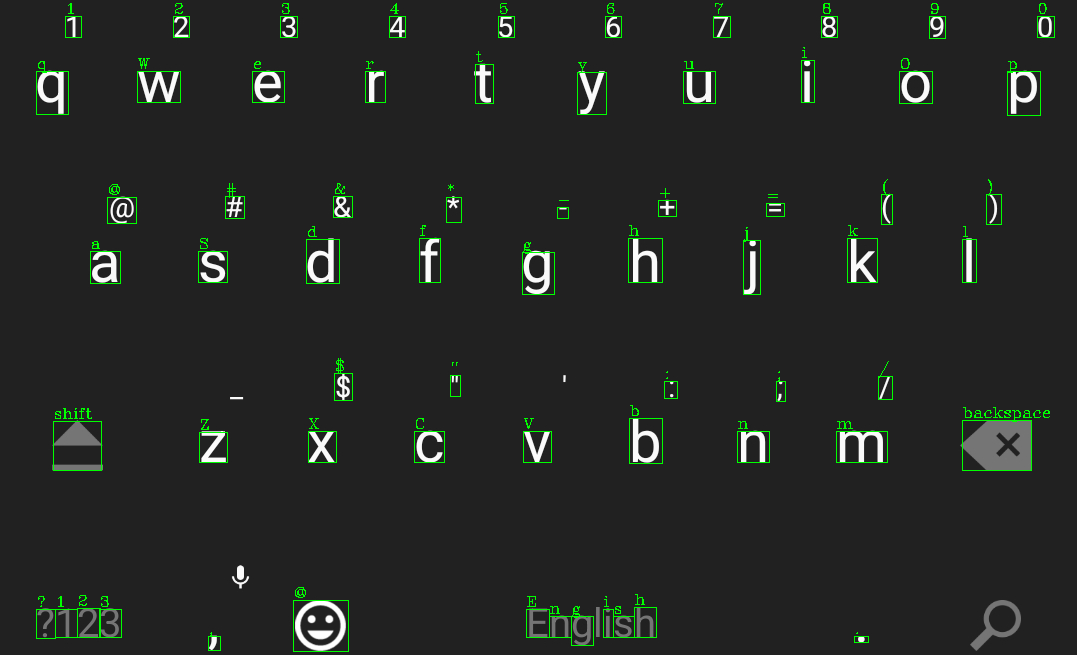
\includegraphics[width=1\textwidth]{img/design/postprocessing-layout-qwerty-false-positives.png}
    \vspace{-15pt}
    \caption{The detector can find characters in~a qwerty layout that are not keys.}
    \label{postprocessing-layout-qwerty-false-positives}
\end{figure}

\begin{figure}[!hbt]
    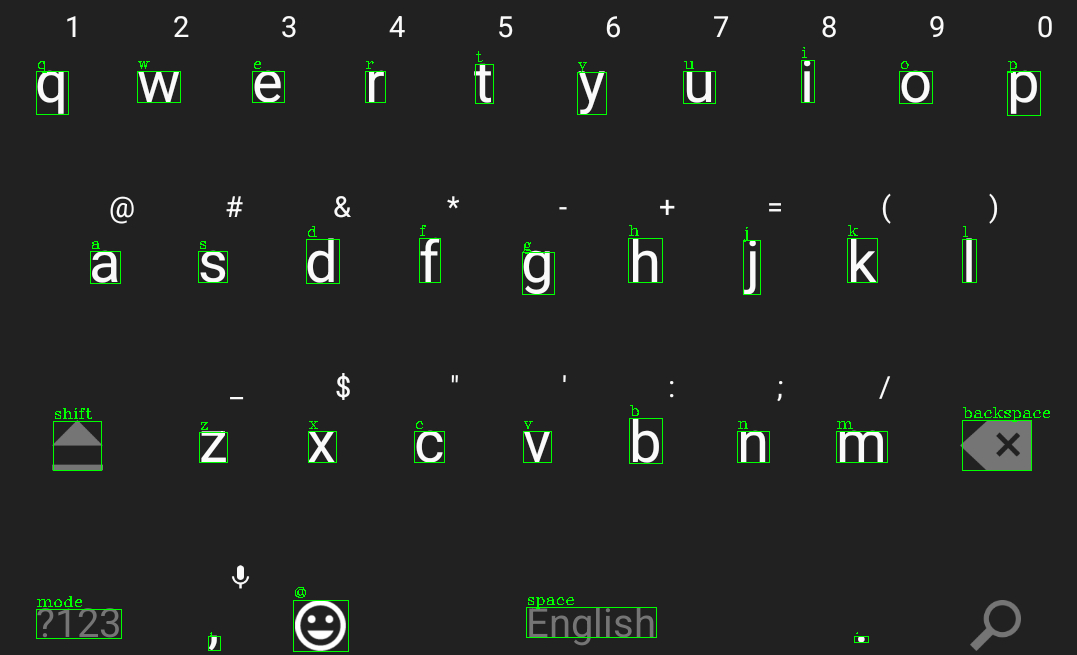
\includegraphics[width=1\textwidth]{img/design/postprocessing-layout-qwerty-removed-false-positives.png}
    \caption{Characters inside the qwerty layout are removed during the post-processing. The numbers above the top row are removed as well due to a margin added to the layout box for this very reason. Characters can be even horizontally outside as the right parenthesis in~the middle row demonstrates which is another reason for the margin.}
    \label{postprocessing-layout-qwerty-removed-false-positives}
\end{figure}

\subsection{Icons processing}
\label{postprocessing-icons}
Detected icons are processed after the layout and keywords are already known. This helps with icon validation and improves false positives detection. Generally, either a keyword or an icon is displayed on~a special key, so a recognized keyword might be an indication of~an invalid icon detection. Therefore, the keyword takes precedence and if it is detected, the icon is ignored. Also, the icon position is taken into~consideration relative to~the layout. Unfortunately, only the qwerty layout offers more or less standardized special key positions, so in~the case of~other layouts, simply the icons with~the highest detection confidence scores are used. The following describes the additional qwerty layout checks or other nuances for~each icon of~interest:

\begin{itemize}[topsep=0pt,itemsep=-1.5pt,partopsep=6pt]
  \item \textbf{Backspace} --- The key should be to~the right of~a qwerty layout so~it accepts the best only among such detections.
  \item \textbf{Enter} --- The check behaves exactly the same as for backspace.
  \item \textbf{Shift} --- The expected and preferred position is to~the left of~the \say{z} key. It might not necessarily be there, though. Next, it looks among those below \say{asd...} row. If not even there, the last check is anywhere to~the left of~the qwerty layout. It is not expected for~a shift to be anywhere else.
  \item \textbf{Tab} --- Tab is the most constraint special key. It is accepted only on~a qwerty layout and only in~its expected position which is left to~the \say{q} key. Thus, the rule of~keyword precedence works differently here. Retrospectively, the position of~the tab keyword is checked and it is removed if it is not correctly placed. This makes the icon the preferred choice, however, also only in~the right position.
  \item \textbf{Space} --- Similarly to~the tab key, the icon can take precedence if it is better positioned. Should the keyword be in~the bottom part of~the keyboard, any space icon is ignored. On~the contrary, the best icon is used with~the preference of~being below the bottom qwerty row.
\end{itemize}

\subsection{Special characters processing}
\label{postprocessing-special-chars}
There is only one pattern searched for among the special characters and it is !@\#\$\%\^{}\&*(). This sequence can be found above the qwerty layout or in~special character layouts. Other special characters are not part of~any rules and from those, only the most confident detection is used. Concerning the pattern, there exists a special case for qwerty layouts. Usually, the special characters above qwerty are on~the same keys as~numbers, where numbers are the main characters. For that reason, the existence of~a number line above the top qwerty row must be checked. If it is present, the special character line is ignored. Moreover, any special characters above the number line, special character line, or top qwerty row are removed as~those are considered the topmost keys in~qwerty layout keyboards.

\subsection{Canny detections processing}
\label{postprocessing-canny}
The objective is to find missing special keys. Unfortunately, too many unknowns limit this task. To~begin with, non-qwerty layouts tend to~have special keys anywhere so this action is constrained only to~qwerty layouts. Moreover, tab or caps~lock keys are not very common on~smartphones and generally on~touch screens, hence it is not even safe to assume their existence. Concerning enter and backspace, they should be present almost always and also the position ought to be to~the right of~the layout. However, their \emph{y}~position is the problem. The backspace key can be at~the top on~physical keyboards, at~the bottom on~smartphones, or even anywhere in~between depending on~the keyboard UI design. The same goes for~enter key which has the usual middle position but that is not a rule as~well. This leaves only shift and space keys. The space is one of~the main reasons for the edge detection as~it can be blank without any text or icon and there is no other way to~recognize it. In addition, it can be recognized quite easily as~it has its fixed position at~the bottom in~the middle and is significantly wider than all other keys. Then the shift key usually sticks to its position to~the left of~the bottom layout row. Furthermore, if it is not so, it is unlikely another key has its place. Thus, it can be relatively safely guessed that the found bounding box is indeed a shift. However, both space and shift key guessing occurs only if the corresponding key has not been found.

The input for this process are results of~the detection from section~\ref{design-classical-algorithms}. The accuracy might vary from very precise to~a lot of~noise bounding boxes which is the downside of~a method with fixed parameters. Therefore, filtration is necessary. As~the special keys are bigger than the character layout keys, the median size is computed and any smaller bounding box is removed. Furthermore, only bounding boxes from the bottom left quarter of~the image are considered as~neither of~the keys is expected to~be elsewhere. An example of~filtered bounding boxes is shown in~figure~\ref{demo-canny}. Once the filtration is complete, the bounding boxes matching the expected coordinates are selected as~the special keys.

\begin{figure}[hbt]
    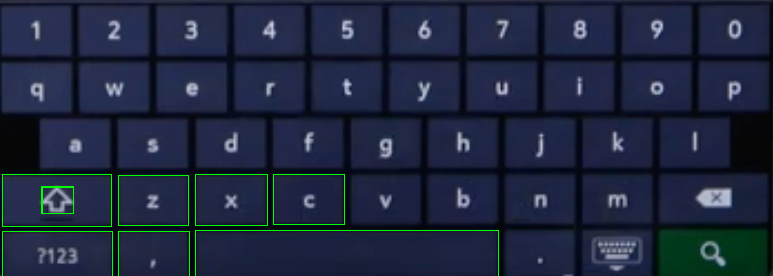
\includegraphics[width=1\textwidth]{img/design/demo-canny.png}
    \caption{Canny detection targets shift and space keys which are constrained to~the bottom left quarter of~the image.}
    \label{demo-canny}
\end{figure}

\section{Final detection process}
\label{design-final-detection-process}
So far, individual parts of~the detection have been described. The whole process is summarized in~figure~\ref{detection-flow-chart}. The image processing starts with feeding the input image to~a trained YOLOv7 keyboard detection neural network model as outlined in~section~\ref{design-keyboard}. The output can be either used as a result of the required individual keyboard detection task or fed as input to~the subsequent character detection. On~the detected keyboard region is simultaneously run character detection using trained YOLOv7 model and Canny edge detection described in~sections~\ref{design-nn-chars} and~\ref{design-classical-algorithms}. The results of~these two detections are then processed in~the final post-processing phase presented in~section~\ref{design-keys-postprocessing}. The final results are bounding boxes with their confidence scores for recognized characters and keyboard in~JSON format. Optionally, images with rendered bounding boxes can be saved as well. The solution is very modular and it is easy to~switch or retrain a model if needed as~well~as include any additional post-processing. A~recognition running script is provided with the options of running full or partial (just keyboard or no post-processing) recognition.

\begin{figure}[hbt]
    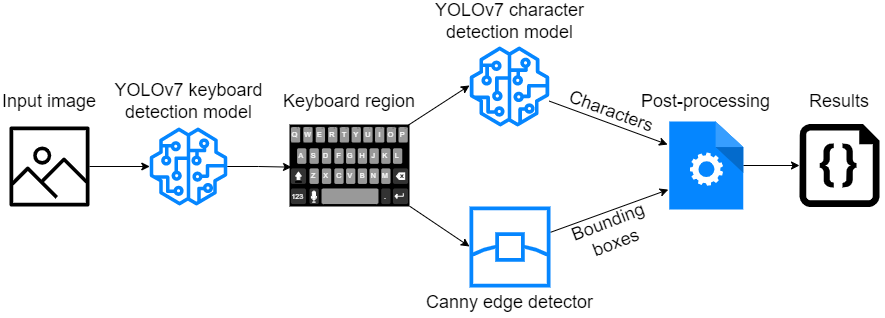
\includegraphics[width=1\textwidth]{img/design/detection-flow-chart.png}
    \caption{Flow of the image recognition process}
    \label{detection-flow-chart}
\end{figure}

The image processing is also visually demonstrated by the following figures. As~an example is used one of~the images from the validation dataset. It illustrates changes done by~each recognition stage and also several post-processing corrections. The first step of~the process which is the keyboard region detection in~the input image is shown in~figure~\ref{demo-detection-keyboard}.

\begin{figure}[hbt]
    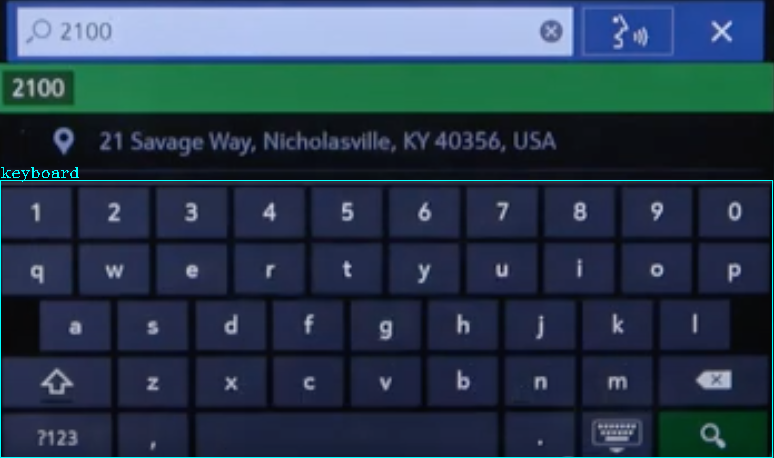
\includegraphics[width=1\textwidth]{img/design/demo-detection-keyboard.png}
    \caption{A keyboard region is detected in~the input image using the YOLOv7 model.}
    \label{demo-detection-keyboard}
\end{figure}

In~the next step, the detected keyboard region is used as~input for the detection of~keys. Figure~\ref{demo-detection-chars} depicts single-character detection results. This detection is run in~parallel with the Canny edge detection described in~section~\ref{postprocessing-canny}. As~can be seen, the detector made some mistakes. It did not recognize characters \hbox{e, i, a, s, l} and has false positive detections for~tab and~Q character at~the bottom right corner. In~addition, it incorrectly classified o~as~0. Other than that, the detections are accurate. There can also be noticed sequence ?123 which stands for a~keyboard mode changing key. It is up to the post-processing algorithm to find it.

\begin{figure}[!hbt]
    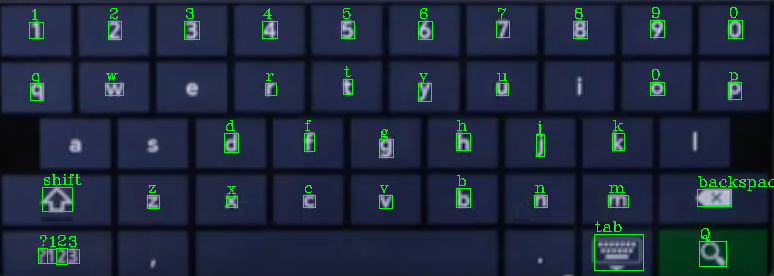
\includegraphics[width=1\textwidth]{img/design/demo-detection-chars.png}
    \caption{Individual characters are detected in~the keyboard using the YOLOv7 model.}
    \label{demo-detection-chars}
\end{figure}

Next, figures~\ref{demo-postprocessing} and~\ref{demo-full-postprocessing} show the post-processing phase. In~figure~\ref{demo-postprocessing} the algorithm computed the missing characters (cyan bounding boxes) and also managed to correct \hbox{the o vs. 0} mistake. Moreover, no rule for the false positive tab and Q was matched so they were removed. Furthermore, the~mode sequence was found and converted to a new key bounding box.

\begin{figure}[hbt]
    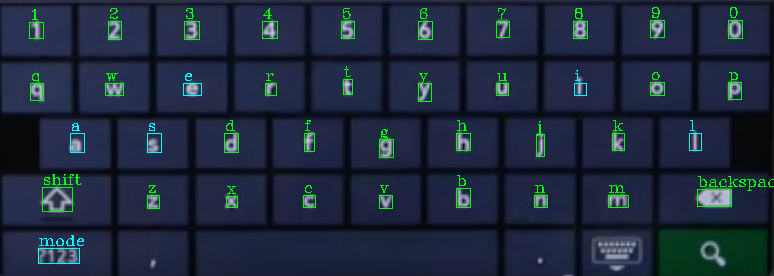
\includegraphics[width=1\textwidth]{img/design/demo-postprocessing.png}
    \caption{Character detections are corrected and missing characters are computed in~the post-processing phase.}
    \label{demo-postprocessing}
\end{figure}

In~figure~\ref{demo-full-postprocessing} can be seen the final post-processing result including the Canny detections. It differs from the figure~\ref{demo-postprocessing} in~that it has the space key recognized. Moreover, the computed keys are not visually distinguished.

\begin{figure}[!hbt]
    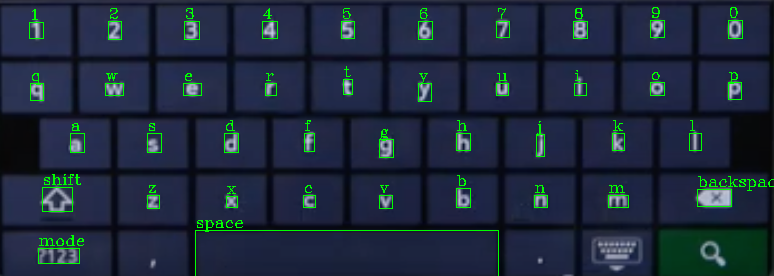
\includegraphics[width=1\textwidth]{img/design/demo-full-postprocessing.png}
    \caption{The post-processing is completed by~incorporating the Canny detection results, namely the space key.}
    \label{demo-full-postprocessing}
\end{figure}

As~already mentioned, the example image comes from the validation dataset. Therefore, to~visually show the recognition accuracy, figure~\ref{demo-evaluation} illustrates the detected and expected keys. The green bounding boxes are the detected ones while the yellow show the expected coordinates. Almost all characters/keys were recognized and the overlap with the ground truth is very good. However, there can be noticed two undetected magenta bounding boxes for~dot and comma characters. Finally, after transforming the detections back to~the original image, figure~\ref{demo-full-detection} depicts the complete keyboard recognition result.

\begin{figure}[!hbt]
    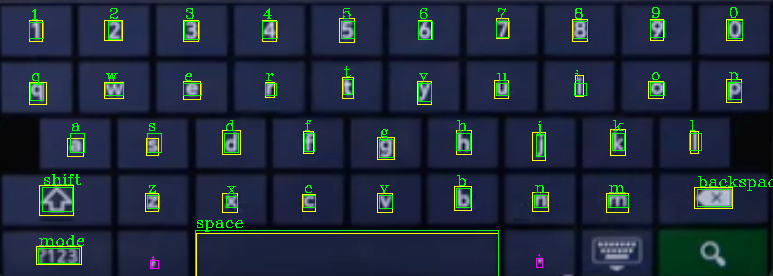
\includegraphics[width=1\textwidth]{img/design/demo-evaluation.png}
    \caption{The detected keys (green) match very well the expected ones (yellow).}
    \label{demo-evaluation}
\end{figure}

\begin{figure}[!hbt]
    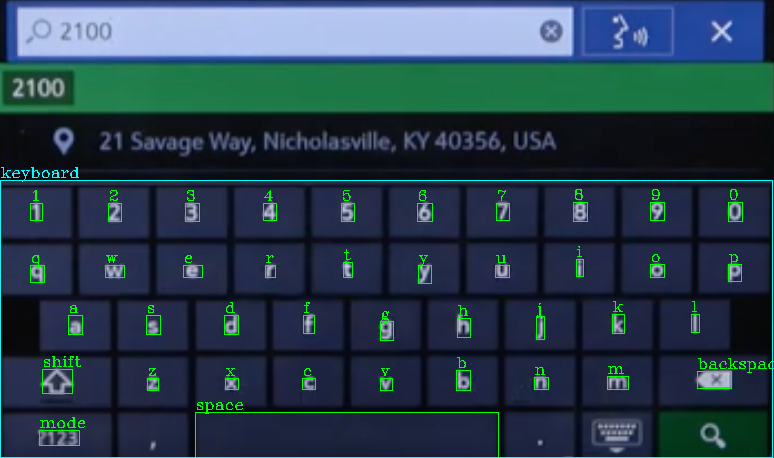
\includegraphics[width=1\textwidth]{img/design/demo-full-detection.png}
    \caption{Fully processed image as~a result of~the image recognition}
    \label{demo-full-detection}
\end{figure}
